\section{Neural Geometry Fields (NGFs)}\label{Sec:MainPart}

The pipeline used by Neural Geometry Fields can be divided into three distinct stages. 

First, a base mesh $\Sigma$ is input and partitioned into quadrangular patches. 
From this, a trainable feature field $\Psi : \Sigma \rightarrow \mathbb{R}^F$ is constructed, where each patch is associated with a set of features that describe its surface properties. 
In the second stage, these features, along with the 3D positions of the mesh, are fed into a neural network to compute the displacement for each point on the mesh. 
The displacements are then applied to the base mesh, resulting in a transformed conventional triangle mesh. 
Finally, the feature field and patches are optimized using an inverse rendering algorithm. 

In the following sections, each stage will be explored in greater detail, with an example provided to further clarify the process. 





\subsection{Surface Partitioning into Patches}

To represent a surface, the base mesh $\Sigma$ is partitioned into quadrilateral patches $\sigma$ by greedily merging adjacent triangles into near-rectangular quads (see Fig.~\ref{fig:surface_processing_pipeline}\,(a)--(b)). 
This simplification step reduces topological complexity and removes non-manifold configurations, enabling a more compact and regular representation of the geometry. 
This reduces the number of patches compared to a purely triangular mesh and simplifies the interpolation domain for further processing. 
\usetikzlibrary{calc, shapes.geometric, arrows.meta, decorations.pathreplacing}
\begin{figure}[ht]
  \centering
  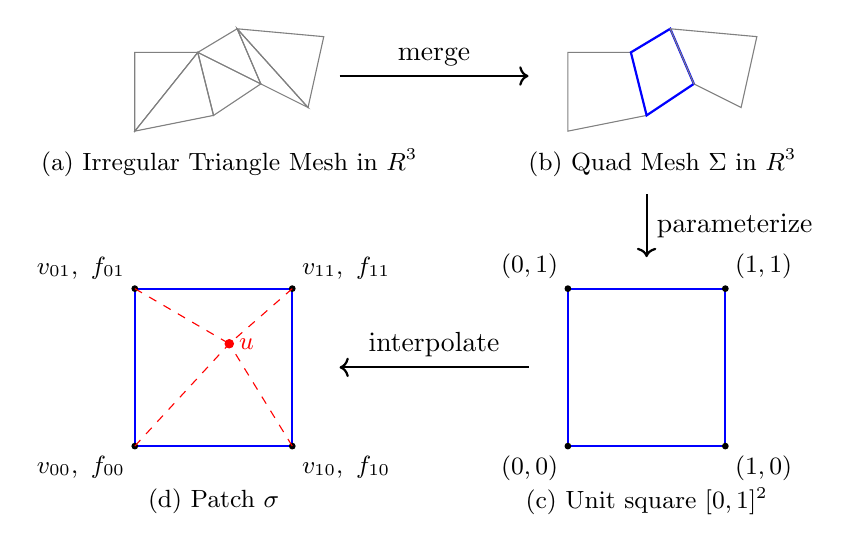
\begin{tikzpicture}

    % === Triangle Mesh (Left) ===
    \begin{scope}
      \coordinate (A) at (0,0);
      \coordinate (B) at (1,0.2);
      \coordinate (C) at (0.8,1);
      \coordinate (D) at (0,1);
      \coordinate (E) at (1.6,0.6);
      \coordinate (F) at (1.3,1.3);
      \coordinate (G) at (2.2,0.3);
      \coordinate (H) at (2.4,1.2);

      \draw[gray] (A) -- (B) -- (C) -- cycle;
      \draw[gray] (A) -- (C) -- (D) -- cycle;
      \draw[gray] (B) -- (E) -- (C) -- cycle;
      \draw[gray] (C) -- (E) -- (F) -- cycle;
      \draw[gray] (E) -- (G) -- (F) -- cycle;
      \draw[gray] (F) -- (G) -- (H) -- cycle;
      \node at (1.2, -0.4) {\small (a) Irregular Triangle Mesh in $\mathbb{R}^3$};
    \end{scope}

    % === Merge Arrow ===
    \draw[->, thick] (2.6,0.7) -- (5.0,0.7) node[midway, above] {merge};

    % === Quadrilateral Mesh (Middle) ===
    \begin{scope}[xshift=5.5cm]
      \coordinate (A) at (0,0);
      \coordinate (B) at (1,0.2);
      \coordinate (C) at (0.8,1);
      \coordinate (D) at (0,1);
      \coordinate (E) at (1.6,0.6);
      \coordinate (F) at (1.3,1.3);
      \coordinate (G) at (2.2,0.3);
      \coordinate (H) at (2.4,1.2);

      \draw[gray] (A) -- (B) -- (C) -- (D) -- cycle;
      \draw[blue, thick] (B) -- (E) -- (F) -- (C) -- cycle; % highlighted patch
      \draw[gray] (E) -- (G) -- (H) -- (F) -- cycle;

      \node at (1.2, -0.4) {\small (b) Quad Mesh $\Sigma$ in $\mathbb{R}^3$};
    \end{scope}

    % === Down Arrow to Unit Square ===
    \draw[->, thick] (6.5,-0.8) -- (6.5,-1.6) node[midway, right] {parameterize};

    % === Unit Square ===
    \begin{scope}[xshift=5.5cm, yshift=-4.0cm]
      \draw[blue, thick] (0,0) rectangle (2,2);
      \filldraw[black] (0,0) circle (1pt) node[anchor=north east] {\small $(0,0)$};
      \filldraw[black] (2,0) circle (1pt) node[anchor=north west] {\small $(1,0)$};
      \filldraw[black] (0,2) circle (1pt) node[anchor=south east] {\small $(0,1)$};
      \filldraw[black] (2,2) circle (1pt) node[anchor=south west] {\small $(1,1)$};
      \node at (1,-0.7) {\small (c) Unit square $[0,1]^2$};
    \end{scope}

    % === Left Arrow to Feature Field ===
    \draw[->, thick] (5.0,-3) -- (2.6,-3) node[midway, above] {interpolate};

    % === Feature Field (Right) ===
    \begin{scope}[yshift=-4.0cm]
      \draw[blue, thick] (0,0) rectangle (2,2);

      % Corner features (bold vectors), with f00 label moved outward
      \filldraw[black] (0,0) circle (1pt) node[anchor=north east] {\small $\bm{v_{00}},\ \bm{f_{00}}$};
      \filldraw[black] (2,0) circle (1pt) node[anchor=north west] {\small $\bm{v_{10}},\ \bm{f_{10}}$};
      \filldraw[black] (0,2) circle (1pt) node[anchor=south east] {\small $\bm{v_{01}},\ \bm{f_{01}}$};
      \filldraw[black] (2,2) circle (1pt) node[anchor=south west] {\small $\bm{v_{11}},\ \bm{f_{11}}$};

      % Interpolation point (u)
      \filldraw[red] (1.2,1.3) circle (1.5pt) node[right] {\small $\bm{u}$};

      % Lines from corners to interpolation point
      \foreach \x/\y in {0/0, 2/0, 0/2, 2/2} {
        \draw[dashed, red] (\x,\y) -- (1.2,1.3);
      }

      % Patch label
      \node at (1,-0.7) {\small (d) Patch $\sigma$};
    \end{scope}
    
  \end{tikzpicture}
  \caption{Surface processing pipeline: The irregular triangle mesh is simplified and merged into a quadrilateral mesh $\Sigma$. A quadrilateral patch is extracted, which is then parameterized over the unit square $[0,1]^2$. This parameterization facilitates both geometric and feature field interpolation, with feature values interpolated at the patch's corners and at an arbitrary point $\bm{u}$. Inspired by~\cite{sivaram2024}.}
  \label{fig:surface_processing_pipeline}
\end{figure}
Initially, the mesh is simplified using QSlim, a robust mesh simplification algorithm that preserves essential structures such as holes and intersections. 
Following simplification, adjacent triangles are merged into quads to form a compact base mesh with fewer patches (minimizing $|Q|$) than a purely triangular representation. 
This also simplifies the interpolation domain, facilitating subsequent processing.

Each patch $\sigma$ must be diffeomorphic to the unit square $[0,1]^2$ (Fig.~\ref{fig:surface_processing_pipeline}\,(c)), meaning there exists a smooth, bijective mapping with a smooth inverse between the patch and the square. 
The four corner vertices of the patch are mapped as follows:

\quad $(0,0) \rightarrow v_{00}$, \quad $(1,0) \rightarrow v_{10}$, \quad $(0,1) \rightarrow v_{01}$, \quad $(1,1) \rightarrow v_{11}$ 

A point $u = (u_x, u_y)$ in the unit square is mapped to a corresponding point on the patch $\sigma$ using bilinear interpolation: 
\[\sigma(u) = (1 - u_y)((1 - u_x)v_{00} + u_x v_{10}) + u_y((1 - u_x)v_{01} + u_x v_{11})\] 

Bilinear interpolation first performs linear interpolation along one axis, then along the other. 
This ensures a smooth and continuous transition across the patch surface. 

In the same way, a scalar or vector-valued feature field defined at the patch corners can be interpolated. 
Given feature values $f_{00}, f_{10}, f_{01}, f_{11}$, the interpolated value $\Psi(u)$ at a point $u$ is: 
\[\Psi(u) = (1 - u_y)((1 - u_x)f_{00} + u_x f_{10}) + u_y((1 - u_x)f_{01} + u_x f_{11})\] 

This method ensures that feature values vary smoothly across the surface (Fig.~\ref{fig:surface_processing_pipeline}\,(d)). 

The complete set of mesh vertices is: 
\[V = \bigcup_{\sigma} \{v_{00}, v_{10}, v_{01}, v_{11} \}\] 

and the corresponding set of feature values is: 
\[F = \bigcup_{\sigma} \{f_{00}, f_{10}, f_{01}, f_{11} \}\] 

Together, these define the base geometry and feature distribution over the mesh. 
This quadrilateral mesh is then used as input to a neural network $\mathrm{MLP}_\theta$, which refines the surface geometry while preserving the topology and structure captured in the simplified base ~\cite{sivaram2024}.





%A regular formula

%\begin{equation}
%    x^2 + y^2 = z^2 
%\end{equation}
%and another one
%\begin{equation}
%    \left\Vert \vec{x} \right\Vert = \sqrt{\sum_{i=0}^{n}{x_i^2 + y_i^2}}.
%\end{equation}

%Here is something with matrices:
%\begin{equation}
%\bf{A}=
%\begin{bmatrix}
%    a & b & c\\
%    d & e & f\\
%\end{bmatrix}^\top.
%\end{equation}

%An some inline stuff $\sum a_i=\bf{B}$.

%\begin{table}
%    \caption[List of Symbols]{Keep a list of symbols in your paper.}
%    \label{tab:ListOfSymbols}
%    \resizebox{\columnwidth}{!}
%    {
%    \input{tabs/ListOfSymbols.tex}
%    }
%\end{table}